%************************************************
\chapter{Perturbation Visualization}\label{perturbation-visualization}
%**************************************

\begin{startbox}{Perturbation visualization perturbs spectral features and measures change in classification predictions}
\item Can be used to investigate well-known spectral power features
\item Can also be implemented through gradients of spectral power features
\item Can be extended to investigate phase features
\end{startbox}


    What features the EEG-decoding ConvNet learns is a scientifically
interesting question and not straightforward to answer. Through
end-to-end training, the networks may learn a variety of features,
including brain-signal features and non-brain-signal features, e.g., eye
movements that correlate to a hand movement. The learned features may be
already known from prior research on brain-signal decoding or represent
novel features that had not been described in the literature. However,
there is no straightforward way to find out what the deep networks have
learned from the brain signals.

    Therefore, we developed an input amplitude perturbation method to
investigate whether the deep networks learn to extract spectral
amplitude features, which are very commonly used in many EEG decoding
pipelines. For example, it is known that the amplitudes, for example of
the alpha, beta and gamma bands, provide class-discriminative
information for motor tasks
\citep{ball_movement_2008,pfurtscheller_evaluation_1979,pfurtscheller_central_1981}.
Hence, it seems a priori very likely that the deep networks learn to
extract such features and worthwhile to check whether they indeed do so.
We also extended this method to investigate the use of phase information
by the networks.

The amplitude perturbation method was developed by me in the context of
this thesis, the phase perturbation method was developed by Kay Hartmann
together with me. Text and figures in this chapter are adapted from
\citep{schirrmeisterdeephbm2017} and \citep{hartmann2018hierarchical}.



\section{Input-Perturbation Network-Prediction Correlation
Map}\label{input-perturbation-network-prediction-correlation-map}


\begin{figure}[ht]
    \myfloatalign
    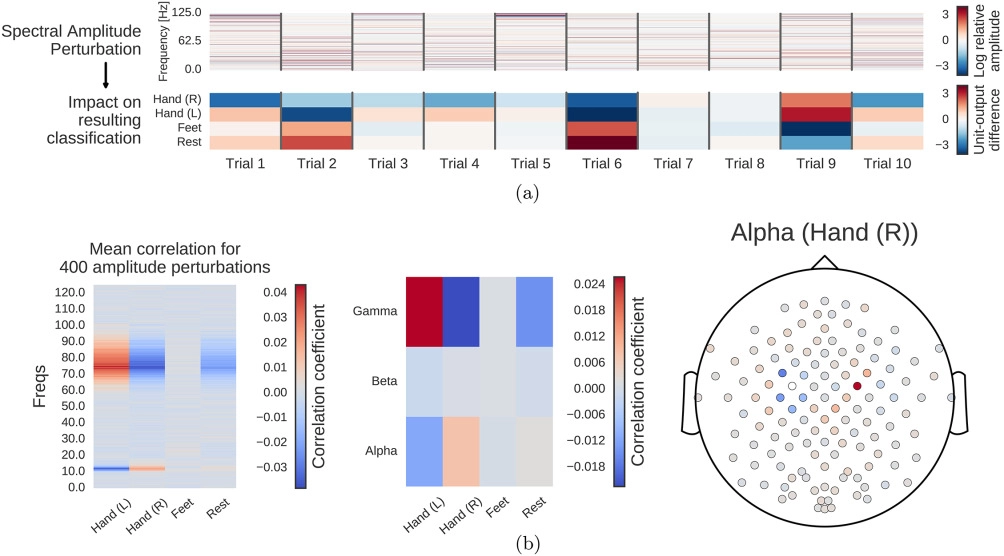
\includegraphics[width=1\linewidth]{images/input-perturbation-overview.png}
    \caption[Computation overview amplitude perturbation]{

\textbf{Computation overview for input-perturbation network-prediction
correlation map.} (a) Example spectral amplitude perturbation and
resulting classification difference. Top: Spectral amplitude
perturbation as used to perturb the trials. Bottom: unit-output
difference between unperturbed and perturbed trials for the
classification layer units before the softmax. (b) Input-perturbation
network-prediction correlations and corresponding network correlation
scalp map for alpha band. Left: Correlation coefficients between
spectral amplitude perturbations for all frequency bins and differences
of the unit outputs for the four classes (differences between
unperturbed and perturbed trials) for one electrode. Middle: Mean of the
correlation coefficients over the the alpha (7--13 Hz), beta (13--31 Hz)
and gamma (71--91 Hz) frequency ranges. Right: An exemplary scalp map
for the alpha band, where the color of each dot encodes the correlation
of amplitude changes at that electrode and the corresponding prediction
changes of the ConvNet. Negative correlations on the left sensorimotor
hand/arm areas show an amplitude decrease in these areas leads to a
prediction increase for the Hand (R) class, whereas positive
correlations on the right sensorimotor hand/arm areas show an amplitude
decrease leads to a prediction decrease for the Hand (R) class. Figure
from \cite{schirrmeisterdeephbm2017}.
}
\label{input-perturbation-overview-figure}
\end{figure}

    To investigate the causal effect of changes in power on the deep
ConvNet, we correlated changes in ConvNet predictions with changes in
amplitudes by perturbing the original trial amplitudes (see
\Cref{input-perturbation-overview-figure} for an overview).
Concretely, the visualization method performs the following steps: 

\begin{enumerate}
\item
Transform all training trials into the frequency domain by a Fourier
transformation 
\item
Randomly perturb the amplitudes by adding Gaussian
noise (with mean 0 and variance 1) to them (phases were kept
unperturbed) 
\item
Retransform perturbed trials to the time domain by the
inverse Fourier transformation
\item
Compute predictions of the deep
ConvNet for these trials before and after the perturbation (predictions
here refers to outputs of the ConvNet directly before the softmax
activation)
\item
Repeat this procedure with 400 perturbations sampled from
aforementioned Gaussian distribution
\item
Correlate the change in input
amplitudes (i.e., the perturbation/noise we added) with the change in
the ConvNet predictions.
\end{enumerate}


To ensure that the effects of our perturbations reflect the behavior of
the ConvNet on realistic data, we also checked that the perturbed input
does not cause the ConvNet to misclassify the trials (as can easily
happen even from small perturbations, see
\citep{szegedy_intriguing_2014}. For that, we computed
accuracies on the perturbed trials. For all perturbations of the
training sets of all subjects, accuracies stayed above 99.5\% of the
accuracies achieved with the unperturbed data.

This method can not only be applied to final predictions, but also to
investigate any intermediate network filter's activations in order to
better understand the intermediate computations of the network.


\section{Gradient-Based
Implementation}\label{gradient-based-implementation}

    An simpler and more computationally efficient way to implement the idea
of testing the sensitivity of the network to spectral amplitude features
is through gradient-based analysis \footnote{This idea was suggested to
  us in personal communication by Klaus-Robert Müller.}. There, we
directly compute the gradient of the output unit with respect to the
amplitudes of all frequency bins of all electrodes of the original
unperturbed trial. To practically implement this, one must first
transform the time domain input signal into the frequency domain and to
a amplitude/phase representation via the Fourier transform. Then, one
can transform the amplitude/phase representation back to the time domain
using the inverse Fourier Transform. Since the inverse Fourier transform
is differentiable, one can backpropagate the gradients from the output
unit through the time domain input back to the amplitudes. The more the
network behaves locally linear around the input, the closer the results
of this variant would be to the original perturbation variant. It is
computationally substantially faster as everything is computed in one
forward-backward pass, without needing to iterate over many
perturbations. The gradient-based method may result in less insightful
visualizations if the prediction function of the network is locally very
nonlinear at a given pint but has an approximately linear relationship
with the spectral amplitudes in a larger neighbourhood around that
point. See works on other saliency/gradient-based visualizations for
discussions in this topic,
e.g. ~\citet{sturmfels2020visualizing}.


\section{Extension to Phase-Based
Perturbations}\label{extension-to-phase-based-perturbations}

\begin{figure}[ht]
    \centering
    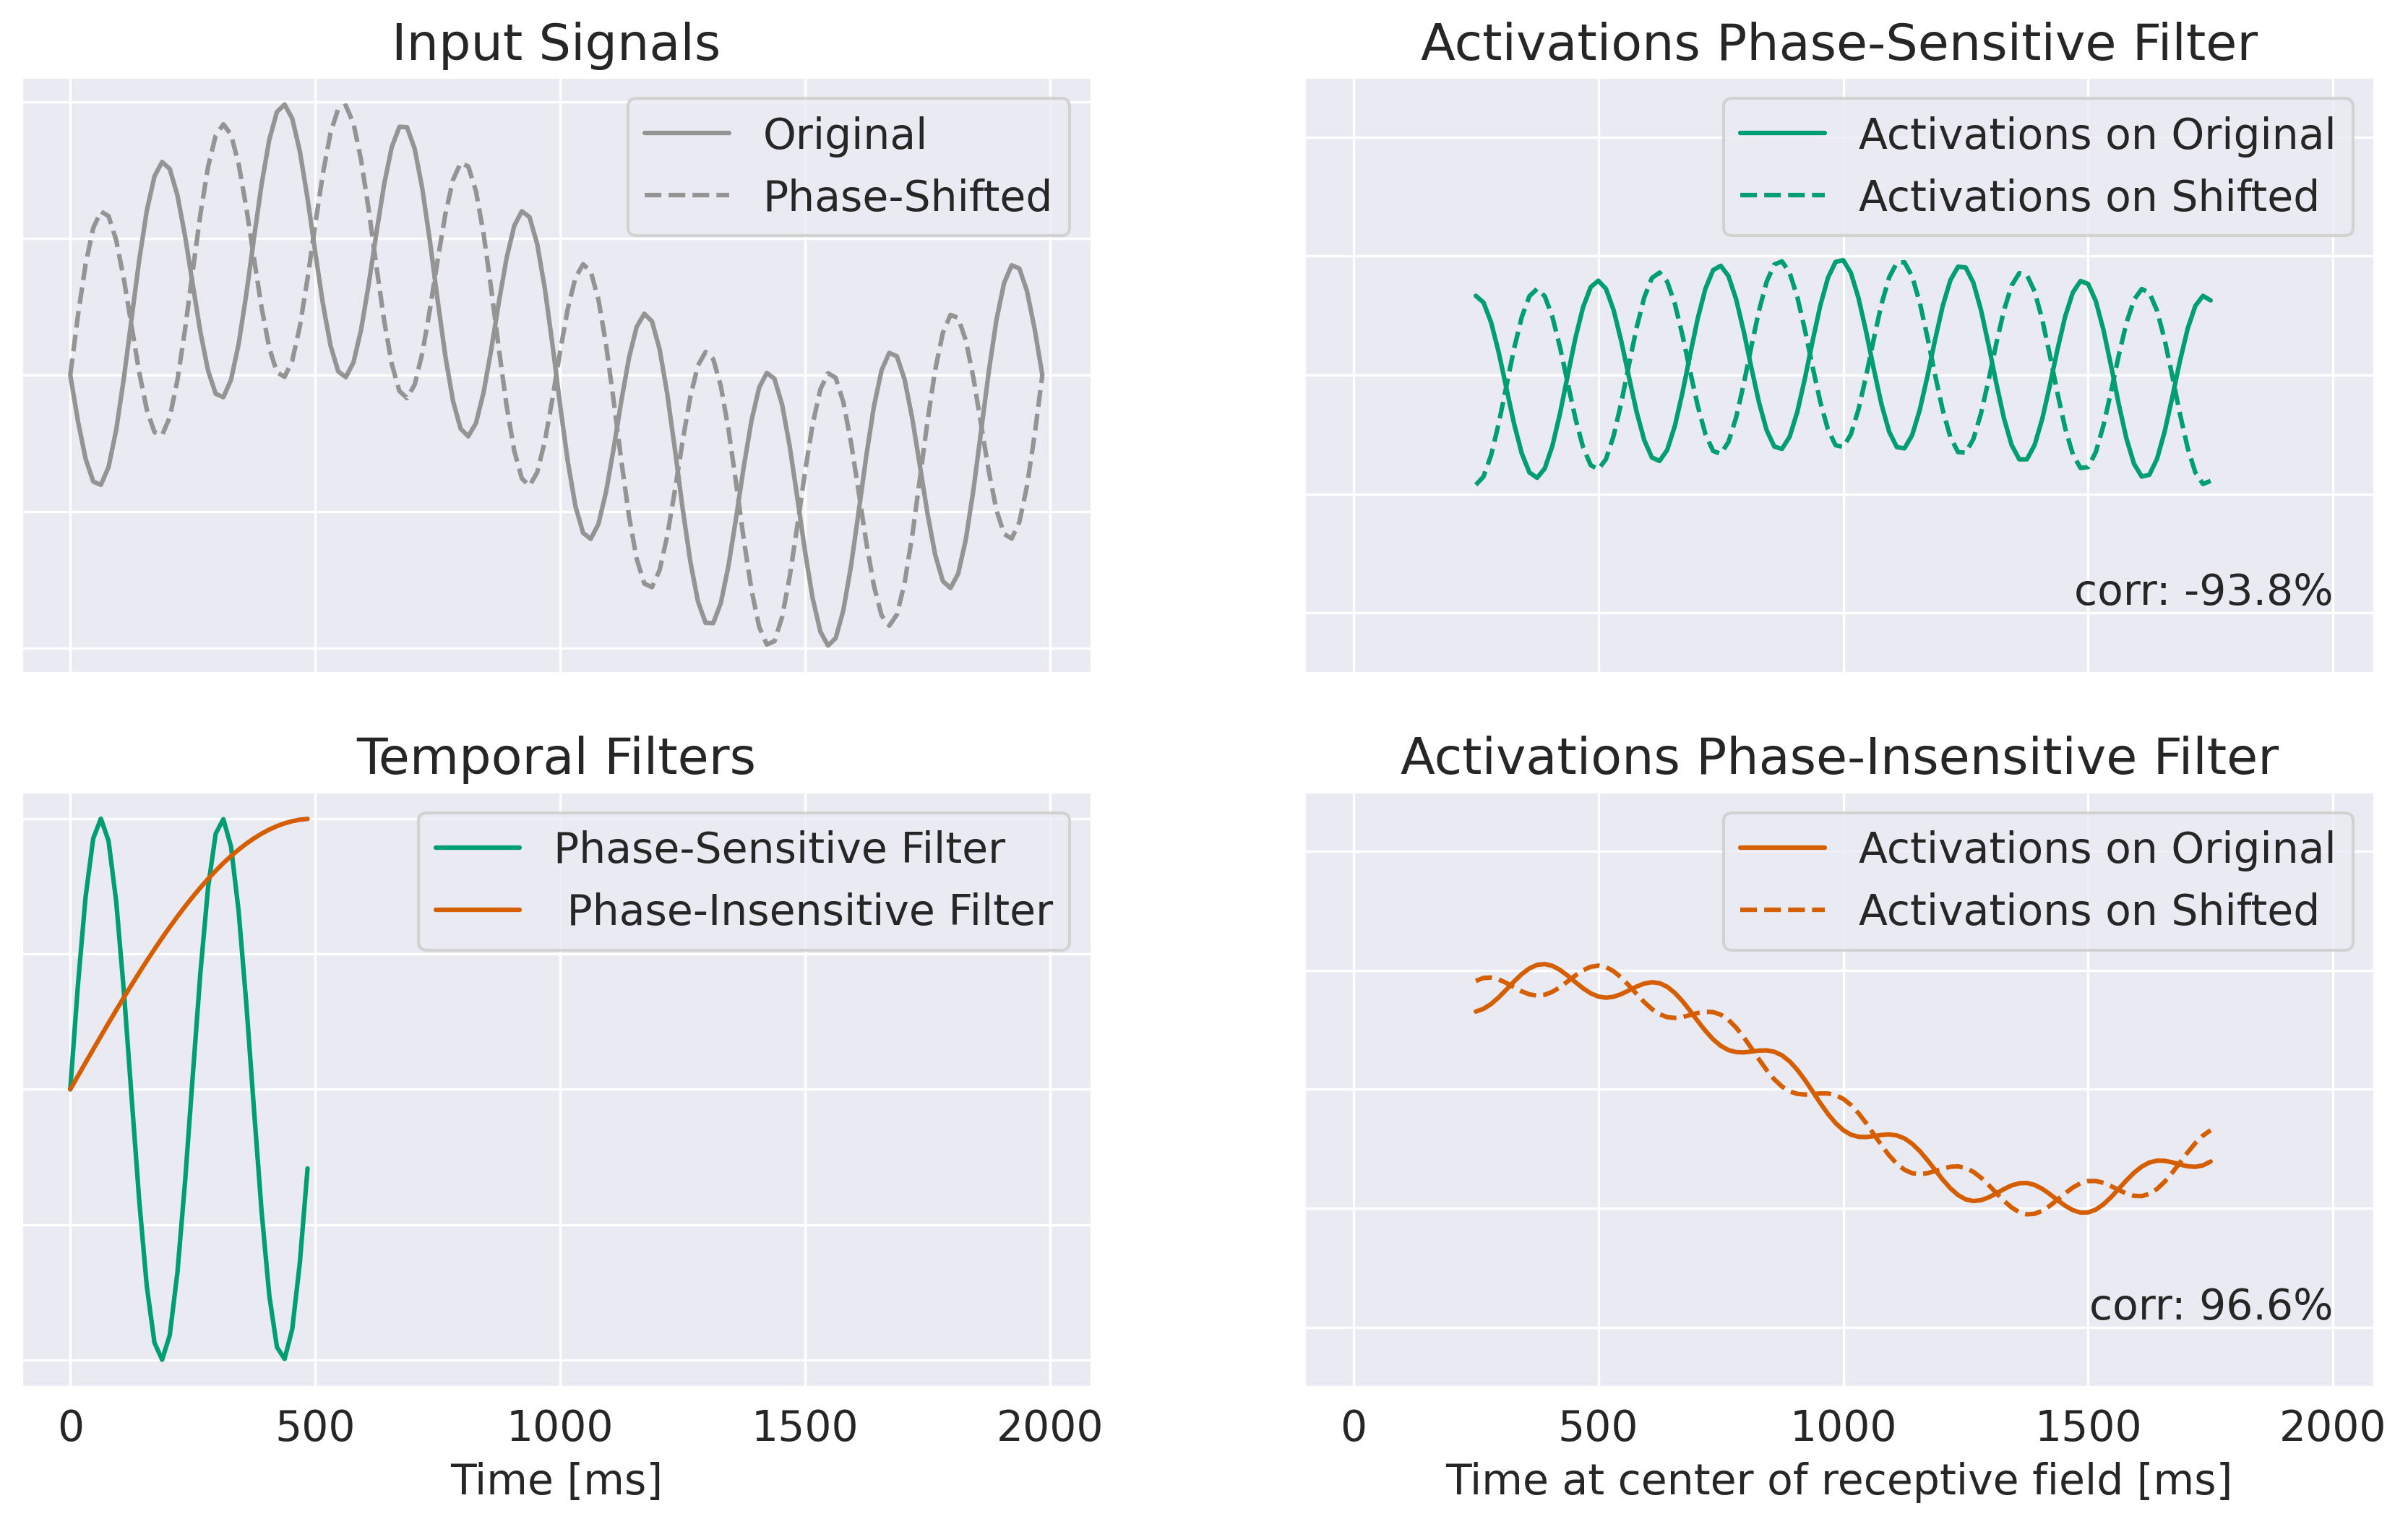
\includegraphics[width=.75\linewidth]{images/phase-perturbation-corr.png}
    \caption[Phase perturbation intuition]{

\textbf{Intuition of the phase perturbation
correlation method.} Top left: two input signals
where the phase of one frequency has been shifted between the two
signals. Bottom left: two temporal filters, one phase-sensitive
and one phase-insensitive to the frequency where the phase was shifted.
Right: activations for the phase-sensitive and
phase-insensitive filter for the original and the shifted signal. The correlation between activations of the phase-sensitive filter is
very low, even negative (-93.8\%), whereas correlation between the
activations of the phase-insensitive filter remains high at 96.6\%. Note
that this simplified example does not illustrate some key mechanisms for
activations to become more generally phase-insensitive such as
nonlinearities and pooling operations.
}
\label{phase-perturbation-corr-figure}
\end{figure}


    The amplitude-perturbation method can also be extended to investigate in
how far networks are affected by changes in phase features. The response
of filters to changes in the phase of certain frequencies was calculated
similarly to the amplitude perturbation correlations. However, because
of the cyclic nature of phase features, the change of activations in a
filter resulting from a phase shift cannot be quantified using the mean
activation difference. When you change the phase of the frequency that a
filter is sensitive to, you won't expect the activations of the filter
to increase uniformly throughout the window. Instead, the activations of
a phase-sensitive filter will probably be temporally shifted by the
phase change. Units of filters whose receptive field contained its
specific phase in the original signal should activate less and units
whose receptive field contains the specific phase in the perturbed
signal should then activate more. Therefore, the original activations
and the activations on the perturbed input should have a decreased
correlation (less than 1). Activation and correlation should remain
similar for phase-insensitive filters.

Phase perturbations were sampled from $p^{P}_{\xi,i}{\sim}N(0,\pi)$.
Perturbed phases $P^{P}_\xi$ were calculated by shifting the phase:
$P^{P}_\xi(X_i)=p^{P}_{\xi,i}+P_\xi(X_i)$. Perturbed signals $X^{P}$
were reconstructed by inverse Fourier transformation. The correlation
between original and perturbation filter activations of a filter $f$
from trial $i$ is denoted by
$\rho_{y_{f,i},y^{P}_{f,i}}=corr(y_{f,i},y^{P}_{f,i})$. Correlations
between phase perturbations $p^{P}_{\xi}$ and filter activity
correlations $\rho_{y_{f},y^{P}_{f}}$ were calculated identically to
amplitude perturbations. The resulting mean absolute phase perturbation
correlations for each layer is denoted as $\varrho^P_{l,\xi}$.

Since we wanted to study only the effect of changing the overall phase
of the signal, independent of the effect of increased or decreased phase
synchronicity across EEG channels, we did not perturb the phase in
channels individually, but applied one phase perturbation of a certain
frequency in all channels equally.

\section{Interpretation and Limitations}
\label{perturbation-visualization-interpretation}


    The perturbation-based visualization reflects network behavior and one
cannot directly draw inferences about the data-generating process from
it. This is because a prediction change caused by an amplitude
perturbation may reflect both learned task-relevant factors as well as
learned noise correlations. For example, increasing the alpha-band
amplitude at electrode C4 (located on the right side), may increase the
predicted probability for right hand movement. That would likely not be
because the alpha amplitude actually increases at C4 during right hand
movement, but because the amplitude \emph{decreases} on C3 \emph{and} is
correlated between C3 and C4. Hence, first subtracting the C4 amplitude
from the C3 amplitude and then decoding associating negative values of
this computation with right hand movement is a reasonable learned
prediction function. And this learned prediction function would cause
the amplitude-perturbation function to show that an alpha increase at C4
causes an increase in the predicted probability for right hand movement.
For a more detailed discussion of this effect in the context of linear
models, see \citep{haufe_interpretation_2014}.

\begin{openbox}
\item Do spectral maps obtained from this visualization show neurophysiologically plausible patterns?
\item What can they reveal about the inner computations of the networks?
\end{openbox}

    

